\documentclass[a4paper, 11pt]{report}
\pdfpagewidth\paperwidth
\pdfpageheight\paperheight
\usepackage[english]{babel}
\usepackage[utf8]{inputenc}
\usepackage[T1]{fontenc}
\usepackage{amsmath,amssymb}
\usepackage{ esint }
\usepackage{ amssymb }
\usepackage{graphicx}
\usepackage{dsfont}
\usepackage{graphics}
\usepackage{float}
\usepackage{tipa}
\usepackage{amsthm}
\usepackage[write,infront,swapnames]{frontespizio}

\theoremstyle{definition}
\newtheorem{definition}{Definizione}[section]

\usepackage{sectsty}
\allsectionsfont{\centering \normalfont\scshape}


%%% Custom headers/footers (fancyhdr package)
\usepackage{fancyhdr}
\pagestyle{fancyplain}
\fancyhead{}											% No page header
\fancyfoot[L]{}											% Empty 
\fancyfoot[C]{}											% Empty
\fancyfoot[R]{\thepage}									% Pagenumbering
\renewcommand{\headrulewidth}{0pt}			% Remove header underlines
\renewcommand{\footrulewidth}{0pt}				% Remove footer underlines
\setlength{\headheight}{13.6pt}


%%% Equation and float numbering
\numberwithin{equation}{section}		% Equationnumbering: section.eq#
\numberwithin{figure}{section}			% Figurenumbering: section.fig#
\numberwithin{table}{section}				% Tablenumbering: section.tab#


%%% Maketitle metadata
\newcommand{\horrule}[1]{\rule{\linewidth}{#1}} 	% Horizontal rule

\title{
		%\vspace{-1in} 	
		\usefont{OT1}{bch}{b}{n}
		\normalfont \normalsize \textsc{École Polytechnique Fédérale de Lausanne} \\ [25pt]
		\horrule{0.5pt} \\[0.4cm]
		\huge Analysis of students performances \\
		\horrule{2pt} \\[0.5cm]
}
\author{
		\normalfont 								\normalsize
        Bollero Francesco, Mariantoni Mattia, Mular Pau, Padovano Federica, Rossi Luca\\[-3pt]		\normalsize
        \today
}
\date{}


%%% Begin document
\begin{document}
\maketitle
\section{Introduction}
In this project we aimed to analyse a database containing information about a sample of students attending a Portuguese language course in two possible different schools ('Gabriel Pereira' or 'Mousinho da Silveira'). For each student there are different attributes related both to their academic performances and to their family context. The table in the next page describes what are the variables that we consider, we can notice that some of them are strictly related with the student academic life (for example "G1","G2","G3","absences" and "studytime") and others tend to describe the student social context, as the family (for example "famsize","Mjob" and "Fjob") and the social life.
 
\begin{figure}[h]\centering
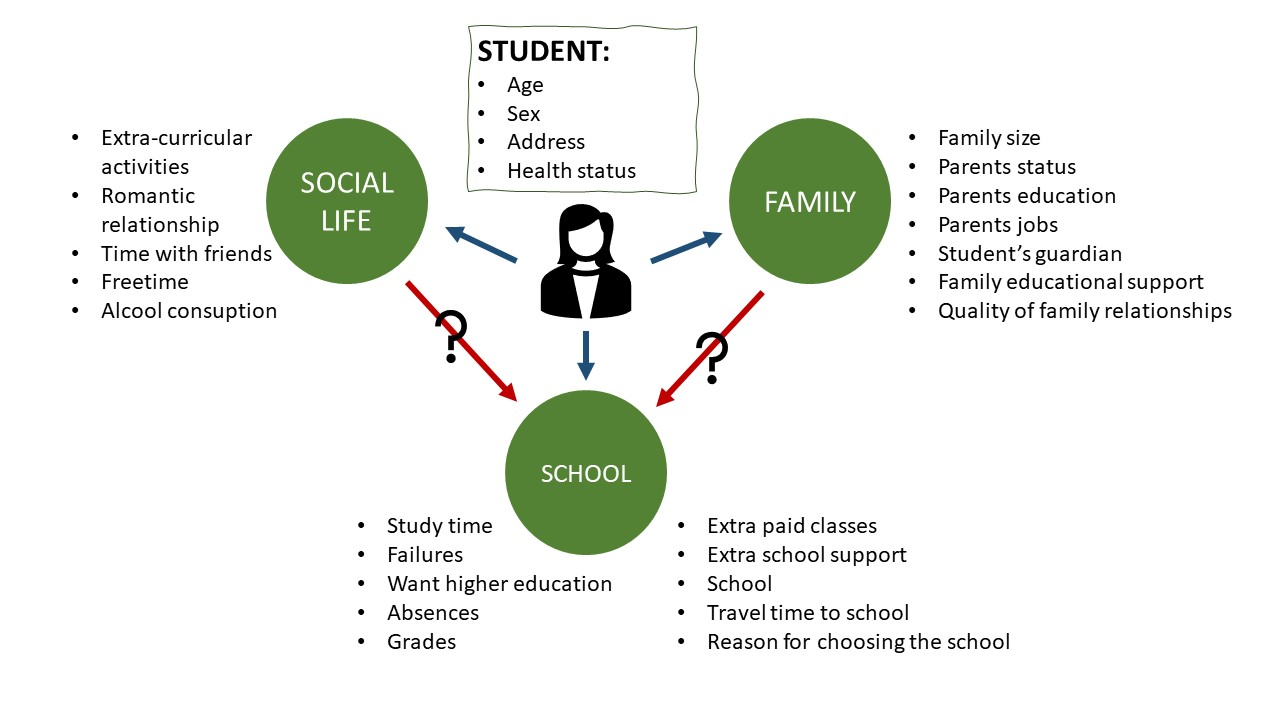
\includegraphics[scale=0.4]{variables.jpg}
\caption{Dataset variables associated with their macroarea.}
\end{figure}

\\After a first glance at the dataset these three variable subsets caught our eyes. In our opinion families and social life impact children's academic path in some way. There are many studies that show how parents with higher educational level have most likely children with higher grades or that want higher education. As the same time, we expect that someone who attends many extra-curricular activities and spend lots of time with friends has less time to study and therefore lower grades. 
\\In this project we want to study the data in order to see if we can credit our opinions or not and to try to predict grades knowing all the other variables. For doing that we want to use statistical visualisations and statistical testing in order to give a more accurate and precise point of view of the analysis .


\flushleft
\noindent
\begin{figure}\makebox[1 \textwidth][c]{       %centering table
\resizebox{1.3 \textwidth}{!}{   %resize table
\begin{tabular}{ |p{2cm}|p{13cm}| }
\hline
Attributes &  Values\\
\hline
school & student's school (binary: "GP" - Gabriel Pereira or "MS" - Mousinho da Silveira)\\
\hline
sex & student's sex (binary: "F" - female or "M" - male)\\
\hline
age & student's age (numeric: from 15 to 22)\\
\hline
address & student's home address type (binary: "U" - urban or "R" - rural)\\
\hline
famsize & family size (binary: "LE3" - less or equal to 3 or "GT3" - greater than 3)\\
\hline
Pstatus & parent's cohabitation status (binary: "T" - living together or "A" - apart)\\
\hline
Medu & mother's education (numeric: 0 - none,  1 - primary education (4th grade), 2 – 5th to 9th grade, 3 – secondary education or 4 – higher education)\\
\hline
Fedu & father's education (numeric: 0 - none,  1 - primary education (4th grade), 2 – 5th to 9th grade, 3 – secondary education or 4 – higher education)\\
\hline
Mjob & mother's job (nominal: "teacher", "health" care related, civil "services" (e.g. administrative or police), "at_home" or "other")\\
\hline
Fjob & father's job (nominal: "teacher", "health" care related, civil "services" (e.g. administrative or police), "at_home" or "other")\\
\hline
reason & reason to choose this school (nominal: close to "home", school "reputation", "course" preference or "other")\\
\hline
guardian & student's guardian (nominal: "mother", "father" or "other")\\
\hline
traveltime & home to school travel time (numeric: 1 - <15 min., 2 - 15 to 30 min., 3 - 30 min. to 1 hour, or 4 - >1 hour)\\
\hline
studytime & weekly study time (numeric: 1 - <2 hours, 2 - 2 to 5 hours, 3 - 5 to 10 hours, or 4 - >10 hours)\\
\hline
failures & number of past class failures (numeric: n if 1<=n<3, else 4)\\
\hline
schoolsup & extra educational support (binary: yes or no)\\
\hline
famsup & family educational support (binary: yes or no)\\
\hline
paid & extra paid classes within the course subject (Math or Portuguese) (binary: yes or no)\\
\hline
activities & extra-curricular activities (binary: yes or no)\\
\hline
nursery & attended nursery school (binary: yes or no)\\
\hline
higher & wants to take higher education (binary: yes or no)\\
\hline
internet & Internet access at home (binary: yes or no)\\
\hline
romantic & with a romantic relationship (binary: yes or no)\\
\hline
famrel & quality of family relationships (numeric: from 1 - very bad to 5 -excellent)\\
\hline
freetime & free time after school (numeric: from 1 - very low to 5 - very high)\\
\hline
goout & going out with friends (numeric: from 1 - very low to 5 - very high)\\
\hline
Dalc & workday alcohol consumption (numeric: from 1 - very low to 5 - very high)\\
\hline
Walc & weekend alcohol consumption (numeric: from 1 - very low to 5 - very high)\\
\hline
health & current health status (numeric: from 1 - very bad to 5 - very good)\\
\hline
absences & number of school absences (numeric: from 0 to 93)\\
\hline
G1 & first period grade (numeric: from 0 to 20)\\
\hline
G2 & second period grade (numeric: from 0 to 20)\\
\hline
G3 & final grade (numeric: from 0 to 20, output target)\\
\hline
\end{tabular}
}
}
\caption{\label{fig:text3}Variables meaning}
\end{figure}


We also decide to split our work in four different points answering different questions:
\begin{enumerate}
\item What's the correlation between variables? Do the grades follow a normal distribution ?
\item Which is the capacity of different variables to explain the grades ?
\item Can we train a model to predict grade based on the other variables ?
\end{enumerate}
and for each point we used different statistical methods.


\section*{1. Correlations and Hypothesis testing}


\begin{itemize}
\item Correlation between Study time and Grades

\begin{figure}[h]\centering
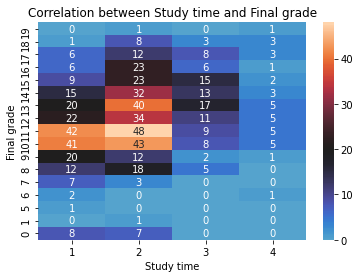
\includegraphics[scale=0.5]{g3-st.png}
\caption{Study times - Final grades.}
\end{figure}


\item Correlation between Sex and academic performances


\item Correlation between age and Final grade


\item Correlation between Student family and grades


\end{itemize}




\section*{1. Correlations and Hypothesis testing}

\section*{3. Grades}


\section*{4. Machine Learning}

All the models have been trained with a 80 to 20 percentage split for training to testing and implemented using the Sklearn library.

\subsection*{Baseline}
The baseline is a constant prediction model which outputs always the most frequent class ( in our dataset is 11 ), this achieves an accuracy of 16 percent.
\subsection*{Logistic Regression}
Logistic regression is a statistical model that in its basic form uses a logistic function to estimate the probabilities for a multivariate dependent variable: $$p=\frac{1}{1+b^{-\left(\beta_{0}+\beta_{1} x_{1}+\beta_{2} x_{2}+\cdots+\beta_{m} x_{m}\right)}}$$
Our model with L2 loss and balanced weights achieved an accuracy of 10.7 percent. 
\subsection*{Random Forest}
Random forests are an ensemble learning method, used for classification in this case, that operates by constructing a multitude of decision trees at training time and correct for decision trees' habit of overfitting to their training set. Our model with max depth of a tree equal to 2 achieved an accuracy of 12.3 percent.
\subsection*{XGboost}
XGboost is a gradient boosting is a machine learning technique, used for classification in this case, which produces a prediction model in the form of an ensemble of weak prediction models, typically decision trees. In particular XGboost is also connected to the Newton-Raphson method. Our model with max depth of a tree equal to 3 achieved an accuracy of 23.8 percent.



\end{document}
